\documentclass[conference]{IEEEtran}
\usepackage[T1]{fontenc}
\usepackage{cite}
\usepackage{amsmath,amssymb,amsfonts}
\usepackage{graphicx}
\usepackage{textcomp}
\usepackage{booktabs}
\usepackage{array}
\usepackage[hidelinks,pdfauthor={},pdfsubject={},pdfkeywords={}]{hyperref}
\usepackage{balance}

\renewcommand\IEEEkeywordsname{Keywords}

\begin{document}

\title{Benchmarking Multi-View Tree-Level Oil Palm Bunch Counting Under a Fixed Detector}

\author{Anonymous Authors}

\maketitle

\begin{abstract}
\bfseries In oil palm plantations, each harvest cycle is planned from a per-tree
count of fruit bunches grouped by maturity class, since each class ripens on a
different schedule. Multi-view imaging recovers bunches hidden by occlusion, but
the same bunch then reappears across several side views, so per-image detections
must be aggregated into a per-tree count rather than summed. Comparing methods
for this tree-level aggregation remains underexplored in oil palm.
This paper evaluates five regression counters and eight feature
configurations on 953 oil palm trees and 3,992 side-view images, under two
detection conditions: ground-truth detections, which measure the counters in
isolation, and a fixed YOLO26m detector, which reflects a deployed pipeline. With
ground-truth detections, the best reported counter reaches 98.05\% Class
$\pm$1 accuracy and 92.20\% Tree $\pm$1 accuracy; under the fixed detector both fall
sharply, to 77.48\% and 32.62\%. A tree-level bootstrap places the class-level
gap at 20.57 points (95\% CI 17.20--23.94), while no two counters differ
significantly under fixed inputs on Class $\pm$1 accuracy after multiplicity correction.
Diagnostic matching finds 22.7\% of test bunches undetected in every view,
alongside substantial maturity-class confusion; these diagnostics do not
provide an additive decomposition of the deployed error. The GT advantage
persists in matched cross-validation, four YOLO26 checkpoints, and a separately
trained YOLO11m, whose matched-counter GT gap is 23.94 points.
These results support prioritising detector output quality on this dataset,
while leaving improvements from other counters and detector families open.
\end{abstract}

\begin{IEEEkeywords}
\bfseries\itshape Oil palm, fresh fruit bunch, black bunch census, multi-view counting, object
detection, YOLO, tree-level regression, agricultural computer vision.
\end{IEEEkeywords}

% ---------------------------------------------------------------------------
\section{Introduction}
% ---------------------------------------------------------------------------

Harvest planning in commercial oil palm plantations depends on knowing, for
each surveyed tree, how many fruit bunches belong to each operational maturity
class. The Black Bunch Census (BBC) formalises this requirement into a four-class
count vector, B1 through B4, where each class carries distinct timing and
logistics implications~\cite{ref12}. Automating BBC through image-based counting
would reduce the cost and subjectivity of manual field surveys. An automated
census is therefore useful only if it recovers the full per-class breakdown for
each tree.

Tree-level counting is geometrically harder than image-level
detection~\cite{ref1}. Bunches surround the full circumference of an oil palm,
so a single image misses bunches due to occlusion, viewing angle, or overlapping
fronds. Multi-view acquisition reduces missed bunches by photographing each tree
from four to eight side views, but the same physical bunch then appears in
several images. Fig.~\ref{fig:crossview} illustrates the effect: a single B3
bunch is visible in three adjacent side views of the same tree. Naive summation
of per-image detections counts appearances rather than bunch identities and is
biased upward on this dataset.

\begin{figure*}[!tb]
  \centering
  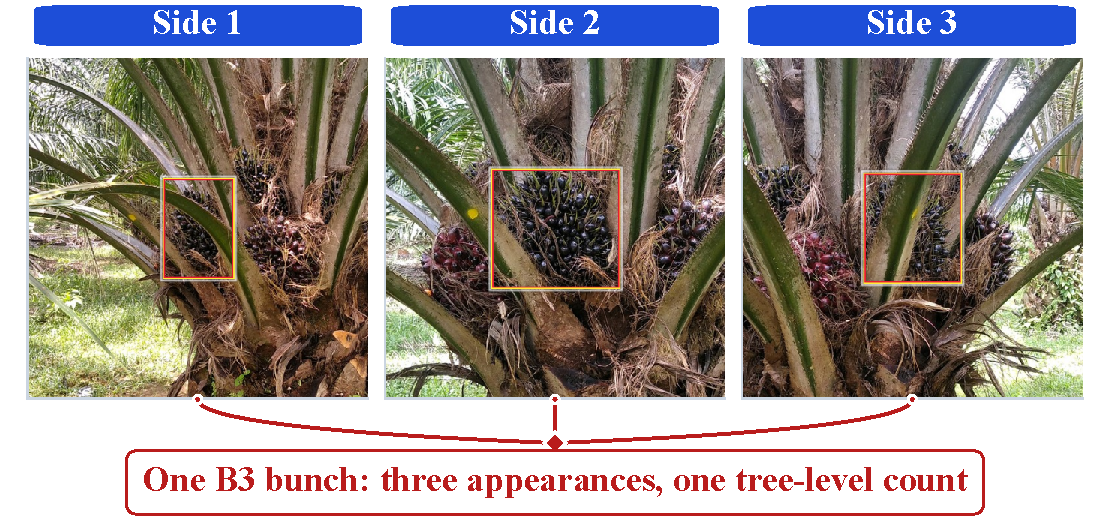
\includegraphics[width=0.86\textwidth]{../figures/paper/fig01_cross_view_linking.pdf}
  \caption{A single physical B3 bunch is visible across three adjacent side
  views. If every per-image detection is counted, three appearances are added
  for one bunch. Tree-level counting must therefore aggregate evidence across
  views rather than sum it.}
  \label{fig:crossview}
\end{figure*}

Multi-view deduplication has been studied across several crops. Mango systems
associated detections across sequential passes using navigation data and canopy
geometry~\cite{ref5}, and apple pipelines built row-level maps from overlapping
two-side scans~\cite{ref6}; a comparative evaluation of the latter reports that
counting errors originate mainly in detection quality rather than in the
aggregation step~\cite{ref7}. Sparse and calibrated viewpoints have been
addressed through correspondence-free triangulation~\cite{ref3} and few-view 3D
reconstruction~\cite{ref4}, and neural-field methods count from unstructured
photographs in a shared 3D representation~\cite{ref8}. Most of these systems
depend on dense sequential overlap, a moving sensor platform, or calibrated
geometry. Their acquisition settings differ from the sparse tree-level
views evaluated here.

Regression-based aggregation instead maps detection statistics to a tree-level
count vector, an approach well established in agricultural
vision~\cite{ref1,ref6,ref7}, with YOLO-style detectors as the standard
front-end~\cite{ref14,ref15}. A counter is typically evaluated only on the
detector output available during the study, so its reported accuracy reflects
that detector's limitations as much as its own quality. Benchmarking counting
methods on their own terms therefore calls for a detection-controlled condition
alongside the realistic one.

Oil palm counting has received less systematic study than apple or mango.
Detectors for fresh fruit bunches (FFB) and maturity classification reach
high image-level accuracy on ripe bunches but show recurring weaknesses on
partially occluded and maturity-ambiguous classes~\cite{refNaftali2024}, with
both two-stage and YOLO-style architectures
explored~\cite{ref9,ref10,ref11,ref13}. The closest public oil palm resource is
a video dataset annotated at the frame level for
detection~\cite{refSuharjito2025}; it carries no tree-level counting labels and
no counting evaluation has been reported on it. No existing benchmark evaluates
tree-level counting strategies for oil palm under both controlled and realistic
detection conditions.

This paper closes that gap by benchmarking tree-level multi-view BBC counting
under two detection conditions on the SawitMVC dataset (953 trees, 3,992
images)~\cite{refIndriani2026}: ground-truth detections, which isolate counter
performance from detector error, and a fixed YOLO26m detector, which reflects a
deployed pipeline. Five regression models and eight feature configurations are
compared, with feature ablation focused on fixed-detector inputs. The
contributions are (1) a controlled-input reference and deployment baseline
with tree-level confidence intervals and paired tests; (2) a feature ablation
quantifying the limited gains observed among the tested representations;
(3) appearance-level error analysis and diagnostic counting rules using
ground-truth identities; and (4) sensitivity analyses across matched
cross-validation, estates, YOLO26 checkpoints, and confidence thresholds.

% ---------------------------------------------------------------------------
\section{Methodology}
% ---------------------------------------------------------------------------

\subsection{Dataset and Task Definition}
\label{sec:task}

The benchmark uses the SawitMVC multi-view dataset: 953 oil palm trees,
3,992 side-view images, four maturity classes (B1, B2, B3, and B4), and 4 to
8 side views per tree. The fixed split contains 716 training trees, 96
validation trees, and 141 test trees. Dataset construction, annotation
protocol, and per-class composition are documented in~\cite{refIndriani2026}.

For tree $i$, the ground-truth target is the count vector
\begin{equation}
  \mathbf{y}_i = [\,y_{i,B1},\;y_{i,B2},\;y_{i,B3},\;y_{i,B4}\,],
\end{equation}
and the prediction is $\hat{\mathbf{y}}_i =
[\,\hat{y}_{i,B1},\ldots,\hat{y}_{i,B4}\,]$. The evaluation unit is the tree,
not the individual image: per-image appearance counts are not valid BBC outputs.

Let $a_{i,c}$ denote the number of detected appearances of class $c$ across
all views of tree $i$. The naive multi-view estimator
\begin{equation}
  \hat{y}_{i,c}^{\text{naive}} = a_{i,c}
\end{equation}
is biased upward whenever a bunch is visible from more than one side. Under GT
annotations, this estimator reaches only 50.00\% Class $\pm$1 Acc and 6.38\%
Tree $\pm$1 Acc on the test split, which motivates learned tree-level
aggregation rather than direct summation.

\subsection{Detection Conditions}

The same counter is fitted separately under two input conditions: annotated
boxes and classes $\rightarrow$ features $\rightarrow$ counts, and cached
detector boxes and classes $\rightarrow$ features $\rightarrow$ counts.

In the \textit{GT detection setting}, the feature extractor reads ground-truth
bounding boxes and classes directly from the annotation files. Counters trained
on these features provide an empirical reference when detections are accurate,
rather than a mathematical upper bound on all counters. In the \textit{fixed-detector setting}, the feature
extractor reads cached YOLO26m~\cite{ref15} predictions from the released
\texttt{y26mv2} checkpoint. The detector was trained on the official 716-tree training
split for 60 epochs (batch size 32, image size 640, patience 60, seed 42;
Ultralytics 8.4.49 in the training log).
Inference uses the repository default confidence threshold of 0.25 and the
standard Ultralytics post-processing settings. A single detector checkpoint is
used for all counter and feature configurations in
Sections~\ref{sec:gt}--\ref{sec:gap}, so any observed difference there comes
from the counter or feature representation rather than from detector
retraining.

Because a claim about detector quality cannot rest on one checkpoint,
Section~\ref{sec:robust} varies the detector along two axes: its operating
point, by sweeping the confidence threshold of the same checkpoint, and its
capacity, by comparing three earlier YOLO26 checkpoints (n, s, and m) against
\texttt{y26mv2}. Those three were trained under an earlier 763/95/95 protocol,
so they are compared on a checkpoint-fair subset, the 590 trees that train
under both protocols and the 64 excluded from gradient training under both.
This subset includes validation trees used during detector development; it is
not an independent test of a second architecture family.
We additionally train YOLO11m on the official 716/96/141 split, using the same
epoch, batch, image-size and seed settings, with 12 data-loader workers and
Ultralytics 8.4.140. Its validation-selected checkpoint is frozen before test
evaluation; Ridge$+F_0$ is refitted on 716 training trees for each input source.
Software versions and architecture-specific defaults differ, so this is a
pipeline comparison, not an isolated causal effect of architecture.

Validation mAP50 follows the COCO convention~\cite{ref16}.

\begin{table}[!tb]
  \centering
  \footnotesize
  \renewcommand{\arraystretch}{1.13}
  \setlength{\tabcolsep}{2.6pt}
  \caption{Detector performance and appearance-level errors.}
  \label{tab:yolo}
  \begin{tabular*}{\columnwidth}{@{\extracolsep{\fill}}lccccccc@{}}
    \toprule
      & \multicolumn{2}{c}{Validation} & \multicolumn{5}{c}{Test split, appearance level} \\
    \cmidrule(lr){2-3}\cmidrule(l){4-8}
    Class & mAP50 & Recall & GT app. & Missed & Wrong & FP & Recall \\
    \midrule
    B1  & \textbf{0.746} & \textbf{0.801} &  252 &  47 &  33 &  58 & \textbf{0.683} \\
    B2  & 0.425          & 0.433          &  496 & 161 & 209 & 158 & 0.254          \\
    B3  & 0.550          & 0.656          & 1409 & 494 &  65 & 393 & 0.603          \\
    B4  & 0.363          & 0.389          &  455 & 262 &  89 &  97 & 0.229          \\
    All & 0.521          & 0.570          & 2612 & 964 & 396 & 706 & 0.479          \\
    \bottomrule
  \end{tabular*}
\par\vspace{3pt}
  \begin{minipage}{\columnwidth}
    \footnotesize\raggedright
    \textit{Note:} Missed/Wrong use GT classes; FP uses predicted classes. Test All recall is pooled; validation All is macro-averaged.
  \end{minipage}
\end{table}

The test block uses the one-to-one IoU matching in Section~\ref{sec:attrib}:
Missed denotes an unmatched annotation, Wrong a matched but misclassified box,
and FP an unmatched detection. Recall requires both localisation and class
correctness; the validation and test blocks use different protocols.

The per-class weakness on B4 and the moderate recall on B3 in
Table~\ref{tab:yolo} are revisited in Sections~\ref{sec:gap}
and~\ref{sec:attrib}.

\subsection{Feature Vectors}

Given either set of detections, observations from all views of a tree are
aggregated into a fixed-length feature vector. The 13-dimensional baseline
$F_0$ contains, for each class $c$, the total count $s_c$, the per-side
maximum $m_c$, and the per-side mean $\mu_c$, plus the number of available
views $n_{\text{views}}$:
\begin{equation}
  F_0 = [\,s_{B1\text{:}B4},\;m_{B1\text{:}B4},\;\mu_{B1\text{:}B4},\;
        n_{\text{views}}\,].
\end{equation}

Four optional groups extend $F_0$: detection confidence (20-dim), spatial
position (8-dim), side distribution (20-dim), and cross-class composition
(6-dim). Together they form the 67-dimensional combined set
\begin{equation*}
  F_{\text{all}} = F_0 \cup \text{conf} \cup \text{spatial}
                      \cup \text{distrib} \cup \text{composition}.
\end{equation*}
For $n_v$ views, let $k_{c,v}$ denote the class-$c$ count in view $v$,
$P_c$ its confidence multiset, $s_c=\sum_v k_{c,v}$, $\mu_c=s_c/n_v$,
and $\sigma_c$ the population SD over all views, including zero-count views.
All denominators use $\varepsilon=10^{-6}$.
Table~\ref{tab:features} defines every entry so that the representation can be
rebuilt from the definition alone. Under GT detections all confidences equal
one, so the confidence group degenerates there and the ablation is run only in
the fixed-detector setting.

\begin{table}[!tb]
  \centering
  \footnotesize
  \renewcommand{\arraystretch}{1.13}
  \setlength{\tabcolsep}{3pt}
  \caption{Definitions of the tree-level features.}
  \label{tab:features}
  \begin{tabular}{@{}l>{\raggedright\arraybackslash}p{0.30\columnwidth}>{\raggedright\arraybackslash}p{0.42\columnwidth}@{}}
    \toprule
    Group (dim) & Entries & Definition \\
    \midrule
    $F_0$ (13) & $s_c$, $m_c$, $\mu_c$, $n_v$
      & total, per-view maximum, and per-view mean detections of class $c$;
        $n_v$ is the number of views, 4 or 8 (global) \\
    \addlinespace[2pt]
    conf (20) & $\Sigma P_c$, $\overline{P}_c$, $\max P_c$, $h_c$, $h^{+}_c$
      & sum, mean, and maximum confidence; counts with $p \ge 0.5$ and
        $p \ge 0.6$ \\
    \addlinespace[2pt]
    spatial (8) & $\overline{cy}_c$, $\overline{A}_c$
      & mean $cy=(y_{\min}+y_{\max})/(2H)$ and mean
        $A=wh/(WH)$, for image width $W$ and height $H$ \\
    \addlinespace[2pt]
    distrib (20) & $\sigma_c$, $\min_v k_{c,v}$,
      $\sigma_c/(\mu_c{+}\varepsilon)$, $|\{v\!:\!k_{c,v}{>}0\}|$,
      $1/(1{+}\sigma_c)$
      & spread and floor across views, coefficient of variation, views holding
        a detection, and view-to-view consistency \\
    \addlinespace[2pt]
    compos.\ (6) & $T$, $s_c/(T{+}\varepsilon)$,
      $s_{B3}/(s_{B2}{+}s_{B3}{+}\varepsilon)$
      & all detections $T=\sum_c s_c$ (global), class shares, and the B3 share
        of the B2/B3 pair (global) \\
    \bottomrule
  \end{tabular}
\par\vspace{3pt}
  \begin{minipage}{\columnwidth}
    \footnotesize\raggedright
    \textit{Note:} Entries repeat for B1--B4 unless marked global. Empty confidence mean/max and area are 0; empty height is 0.5.
  \end{minipage}
\end{table}

Eight feature sets are evaluated: $F_0$, $F_0$+conf, $F_0$+spatial,
$F_0$+distrib, $F_0$+conf+spatial, $F_0$+conf+distrib, $F_0$+distrib+spatial,
and $F_{\text{all}}$.

\subsection{Counter Models and Evaluation Metrics}

Two heuristic baselines are included as reference points. The \textit{naive
sum} sums all detected appearances per class (defined in
Section~\ref{sec:task}). The \textit{global divisor} scales the naive sum by a
single constant fitted separately in each input condition: the ratio of input
appearances to annotated unique bunches over the 716 training trees.
This gives $k=1.891$ for GT inputs and $k=1.793$ for fixed-detector inputs;
neither calibration uses validation or test trees.

Five regression models are evaluated in both detection conditions: Linear
Regression, Ridge~\cite{ref19}, ElasticNet~\cite{ref17}, SVM~\cite{ref20}, and
Random Forest~\cite{ref18}. Each counter maps a tree feature vector
$\mathbf{x}_i$ to the count vector $\hat{\mathbf{y}}_i =
f_{\theta}(\mathbf{x}_i)$.

All fitted counters are trained only on the 716-tree training split with
deterministic seed 42, and continuous outputs are rounded to the nearest
non-negative integer before scoring. All but Random Forest use standardized
features. Ridge uses RidgeCV over $\alpha \in \{0.01,0.1,1,10,100,500\}$;
ElasticNet uses MultiTaskElasticNetCV with 5-fold cross-validation and 3000
maximum iterations; SVM is an RBF SVR in a multi-output wrapper with 3-fold
GridSearchCV over $C \in \{0.1,1,10\}$ and
$\gamma \in \{\text{scale},0.01,0.1\}$; Random Forest uses 200 trees of
maximum depth 10.

These settings preserve the released benchmark. Ridge and ElasticNet scale
the outer training data before their internal CV; SVM scales within its CV
pipeline. Outer test trees never enter these fits. ``Best'' below denotes the
highest observed test score among compared configurations, not a model selected
on an independent validation set.

All counter models are evaluated on the fixed 141-tree test split. Class-level
$\pm 1$ correctness for tree $i$ and class $c$ is
\begin{equation}
  I_{i,c}^{\pm 1} =
  \begin{cases}
    1, & |\hat{y}_{i,c} - y_{i,c}| \leq 1, \\
    0, & \text{otherwise}.
  \end{cases}
\end{equation}

\textbf{Class $\pm$1 Acc} averages this indicator over all test trees and
classes:
\begin{equation}
  \text{Class } \pm 1 \text{ Acc} =
    \frac{1}{4N}\sum_{i=1}^{N}\sum_{c=1}^{4} I_{i,c}^{\pm 1}.
\end{equation}

\textbf{Tree $\pm$1 Acc} is stricter: a tree counts as correct only if all
four class predictions are within $\pm 1$ simultaneously,
\begin{equation}
  \text{Tree } \pm 1 \text{ Acc} =
    \frac{1}{N}\sum_{i=1}^{N}
      \mathbf{1}\!\left(\sum_{c=1}^{4} I_{i,c}^{\pm 1} = 4\right).
\end{equation}

\textbf{Macro MAE} is the mean absolute error averaged over trees and classes,
and \textbf{macro RMSE} is the per-class root mean squared error averaged over
classes; RMSE is reported because a squared penalty exposes the few badly
mis-counted trees that MAE dilutes. \textbf{Signed class bias} is the per-class
mean $\hat{y}_{i,c} - y_{i,c}$; positive values indicate over-counting,
negative values under-counting. Bias is reported alongside accuracy because
operational aggregate yield estimates are sensitive to directional error rather
than absolute error alone. Two whole-tree aggregate measures complete the set:
\textbf{total-count MAE}, the mean of $|\sum_c \hat{y}_{i,c} - \sum_c y_{i,c}|$,
and \textbf{total $\pm$1 Acc}, the fraction of trees whose total bunch count is
within one of the truth. These matter for block-level yield forecasting, where
per-class assignment can be wrong while the total remains
usable.\footnote{Repository link withheld in this anonymous companion.}

\subsection{Uncertainty and Validation Protocol}
\label{sec:stats}

For the main fitted configurations, percentile bootstrap intervals resample
trees ($B=10{,}000$, seed 42); paired intervals reuse the same tree indices.
The release includes intervals for per-class and aggregate metrics. Class
$\pm$1 differences use an exact paired permutation test exchanging model
outcomes within each tree, preserving dependence among its four classes.
All ten counter pairs per condition are tested, with Holm adjustment within
each condition; the seven Ridge feature comparisons against $F_0$ form a
separate family. Unadjusted $p$ and adjusted $p_H$ are distinguished below.
Wilcoxon tests on per-tree macro absolute error and exact McNemar tests on
Tree $\pm$1 outcomes address different endpoints and are reported separately.
Intervals and tests condition on fitted models and do not account for
post-hoc configuration selection or detector retraining. Nonsignificance
does not establish equivalence.

A separate selection check ranks all 40 model/feature candidates in each
condition on the 96 validation trees: highest Class $\pm$1, then lowest
macro MAE, fewer dimensions, and model/feature name as deterministic tie-breaks.
Only training trees enter model fitting; test labels do not select the winner.
This reanalysis uses the historical test set, not newly collected test data.

Repeated stratified 5-fold CV with 5 repeats uses estate and dominant class
jointly for stratification. Matched GT/fixed Ridge$+F_0$ comparisons use
identical folds of the 237 trees outside detector gradient training, fitting
on 189--190 trees per fold. Because this pool includes the detector's 96
validation trees, a stricter check uses only the 141 original test trees
(112--113 training trees per fold). The detector stays frozen. Fold standard
deviations are descriptive, since repeated folds overlap. Cross-estate tests
transfer the counter; the detector was trained on both estates.

% ---------------------------------------------------------------------------
\section{Results and Discussion}
% ---------------------------------------------------------------------------

Section~\ref{sec:gt} reports both detection conditions,
Section~\ref{sec:ablation} tests whether richer features recover the loss, and
Section~\ref{sec:gap} compares the conditions per class.
Section~\ref{sec:attrib} examines detection and aggregation diagnostics,
Section~\ref{sec:robust} tests how far the resulting
claim survives changes of detector, split, and site, and
Section~\ref{sec:rf} explains the one counter that behaves differently.

\subsection{Counting Under the Two Detection Conditions}
\label{sec:gt}

Table~\ref{tab:counting} places both conditions side by side. Under GT
detections, naive appearance summation yields only 50.00\% Class $\pm$1 Acc and
6.38\% Tree $\pm$1 Acc, confirming that duplicate visibility cannot be ignored
and that direct summation is not a viable estimator. The calibrated divisor
recovers most of that loss, and ElasticNet improves further to 98.05\%, so with
accurate detections the counting problem is simple enough for compact
regression models. The four best fitted counters sit within 0.53 percentage
points of each other on Class $\pm$1 Acc and 2.13 points on Tree $\pm$1 Acc,
and their pairwise Class $\pm$1 differences are not significant ($p_H=1$).
ElasticNet exceeds Random Forest by 2.13\,pp (95\% CI 0.89--3.55,
$p=0.0042$, $p_H=0.0376$); SVM also exceeds RF ($p_H=0.0342$).
Section~\ref{sec:rf} examines RF's prediction behaviour.

\begin{table}[!tb]
  \centering
  \footnotesize
  \renewcommand{\arraystretch}{1.13}
  \setlength{\tabcolsep}{3pt}
  \caption{Counting performance with baseline features.}
  \label{tab:counting}
  \begin{tabular*}{\columnwidth}{@{\extracolsep{\fill}}lcccccc@{}}
    \toprule
     & \multicolumn{3}{c}{GT detections} & \multicolumn{3}{c}{Fixed detector} \\
    \cmidrule(lr){2-4}\cmidrule(l){5-7}
    Method & Class $\pm$1 & Tree $\pm$1 & MAE & Class $\pm$1 & Tree $\pm$1 & MAE \\
    \midrule
    Naive sum         & 50.00          & 6.38           & 2.142          & 50.71          & 10.64          & 2.447 \\
    Global divisor    & 95.57          & 86.52          & 0.356          & 70.21          & 22.70          & 1.188 \\
    \addlinespace[2pt]
    ElasticNet        & \textbf{98.05} & \textbf{92.20} & 0.277          & \textbf{76.42} & 29.79          & \textbf{1.043} \\
    SVM               & 97.87          & 91.49          & \textbf{0.266} & 74.82          & 29.08          & \textbf{1.043} \\
    Ridge             & 97.70          & 90.78          & 0.275          & 76.06          & 28.37          & 1.053 \\
    Linear reg. & 97.52          & 90.07          & 0.277          & 75.71          & \textbf{30.50} & 1.048 \\
    Random forest     & 95.92          & 84.40          & 0.365          & 73.23          & 26.95          & 1.110 \\
    \bottomrule
  \end{tabular*}
\par\vspace{3pt}
  \begin{minipage}{\columnwidth}
    \footnotesize\raggedright
    \textit{Note:} Accuracy is in \%; MAE is macro MAE. The divisor is fitted separately per input condition using training trees only.
  \end{minipage}
\end{table}

For the strongest $F_0$ Class $\pm$1 scores, the 95\% bootstrap intervals
are 97.0--99.1\% (GT) and 73.2--79.6\% (fixed).
Moving to cached YOLO26m detections, the best $F_0$ result (ElasticNet,
76.42\%) trails the same counter under GT by 21.63 percentage points (95\% CI
18.44 to 25.00, $p < 0.001$). All five counters stay within a 3.19-point
window, and none of the ten Class $\pm$1 comparisons is significant;
the widest, ElasticNet over Random Forest, gives $+3.19$\,pp
(95\% CI $0.00$ to $+6.38$, $p=0.0628$, $p_H=0.628$). A large drop across
conditions, set against a spread among counters that the test set cannot
resolve, points to the detector output rather than the counter family as the
main source of loss.

The per-class picture is the same whichever counter is used: B1 stays near its
GT ceiling at 95.74--96.45\% Class $\pm$1 Acc, B3 collapses to 55.32--56.03\%,
and B2 (73.76--80.14\%) and B4 (67.38--73.05\%) sit at intermediate losses.
Detection recall alone does not rank these losses: B3 has the largest
counting loss despite higher test recall than B2/B4. Its larger counts and
cross-class confusion also affect the absolute $\pm$1 criterion.

\subsection{Feature Ablation}
\label{sec:ablation}

\begin{table}[!tb]
  \centering
  \footnotesize
  \renewcommand{\arraystretch}{1.13}
  \setlength{\tabcolsep}{3pt}
  \caption{Ridge feature ablation under detector inputs.}
  \label{tab:ablation}
  \begin{tabular*}{\columnwidth}{@{\extracolsep{\fill}}lccccc@{}}
    \toprule
    Features & Dim & Class $\pm$1 & Tree $\pm$1 & MAE & CV Class $\pm$1 \\
    \midrule
    $F_0$        & 13 & 76.06          & 28.37          & 1.053          & 72.70 $\pm$ 2.35 \\
    $F_0$+C      & 33 & 75.89          & 29.79          & 1.059          & \textbf{73.26} $\pm$ 2.36 \\
    $F_0$+S      & 21 & 76.60          & 30.50          & 1.046          & 72.65 $\pm$ 2.37 \\
    $F_0$+D      & 33 & 74.82          & 28.37          & 1.060          & 72.89 $\pm$ 1.96 \\
    $F_0$+C+S    & 41 & 76.24          & 29.08          & 1.059          & 72.40 $\pm$ 2.46 \\
    $F_0$+C+D    & 53 & 76.42          & 29.79          & 1.060          & 72.59 $\pm$ 2.02 \\
    $F_0$+D+S    & 41 & 75.71          & 30.50          & 1.048          & 72.34 $\pm$ 2.33 \\
    $F_{\text{all}}$ & 67 & \textbf{77.48} & \textbf{32.62} & \textbf{1.035} & 72.34 $\pm$ 2.08 \\
    \bottomrule
  \end{tabular*}
\par\vspace{3pt}
  \begin{minipage}{\columnwidth}
    \footnotesize\raggedright
    \textit{Note:} C: confidence; S: spatial; D: distribution. CV: mean $\pm$ fold SD on 237 trees, including detector validation trees. MAE is macro MAE.
  \end{minipage}
\end{table}

Whether enriched features can recover the detector-driven gap is tested by
fixing Ridge and varying the feature configuration (Table~\ref{tab:ablation}).
On the fixed test split the eight configurations run from 74.82\%
($F_0$+D) to 77.48\% ($F_{\text{all}}$) Class $\pm$1 Acc, so the full set gains
1.42 points at class level and 4.25 at tree level over the 13-dimensional
baseline. The CV column repeats the eight feature sets using the protocol
in Section~\ref{sec:stats}.

The gain is not statistically resolved. Paired against $F_0$ it gives
$+1.42$\,pp (95\% CI $-0.53$ to $+3.37$, $p=0.201$, $p_H=1$).
Under cross-validation the eight
feature sets fall inside a 0.92-point band whose fold-to-fold standard
deviation is more than twice as wide, with $F_{\text{all}}$ no longer leading
(Table~\ref{tab:ablation}, last column). No Class $\pm$1 comparison with
$F_0$ is significant after adjustment. This limits the evidence for these
particular feature additions; it does not prove that detector outputs contain
no further useful information or that all counting methods are equivalent.

\subsection{GT vs.\ Fixed-Detector Gap}
\label{sec:gap}

The central comparison is the per-class gap between ideal detections and the
fixed detector, reported with the signed bias of the best configuration in each
condition in Table~\ref{tab:summary}.

The gap is large, at 20.57 percentage points in Class $\pm$1 Acc (95\% CI 17.20
to 23.94, $p < 0.001$) and 59.57 points in Tree $\pm$1 Acc, and it is not
uniform across maturity classes: B1 loses 2.84\,pp, B2 16.31\,pp, B3
36.17\,pp, and B4 26.95\,pp. With the same Ridge$+F_0$ configuration in both
conditions, the gap remains 21.63\,pp (95\% CI 18.44--25.00, $p<0.001$),
so it does not depend on comparing different counter families. The squared-error view
agrees: macro RMSE rises from 0.522 to 1.418 and total-count MAE from 0.979 to
1.787 bunches per tree; total $\pm$1 accuracy is 78.01\% and 48.94\%,
respectively. This is per-tree count error; block-level forecasting
error also depends on cancellation and dependence across trees.

Validation-based selection chooses Ridge$+F_0$ for GT and SVM$+(F_0+\mathrm{conf})$
for fixed inputs. Their test Class $\pm$1 accuracies are 97.70\% and 74.11\%,
respectively: a 23.58-point gap (95\% CI 20.21--27.13, $p<0.001$).
Their Tree $\pm$1 accuracies are 90.78\% and 27.66\%. Thus the large
between-condition difference persists when test scores do not determine
configuration selection.

Bias adds direction to the gap. The fixed-detector Ridge $+ F_{\text{all}}$
pipeline under-counts B2 by 0.078 and B3 by 0.177 bunches per tree, while B4 is
over-counted by 0.071 despite its low recall. A learned counter combines
misses, false positives, and class confusion, so this output bias cannot be
assigned to a single confusion direction. The total signed bias is $-0.170$
bunches per tree; it should be assessed alongside per-tree absolute error
before extrapolating to operational harvest forecasts.

\begin{table}[!tb]
  \centering
  \footnotesize
  \renewcommand{\arraystretch}{1.13}
  \setlength{\tabcolsep}{3pt}
  \caption{Per-class counting performance.}
  \label{tab:summary}
  \begin{tabular*}{\columnwidth}{@{\extracolsep{\fill}}llccccc@{}}
    \toprule
    Configuration & Metric & B1 & B2 & B3 & B4 & All \\
    \midrule
    GT,                     & Acc.\ $\pm$1 (\%) & 100.00  & 99.29   & 93.62   & 99.29   & 98.05 \\
    ElasticNet$+F_0$        & MAE             & 0.050   & 0.227   & 0.603   & 0.227   & 0.277 \\
                            & RMSE            & 0.223   & 0.519   & 0.855   & 0.491   & 0.522 \\
                            & Bias            & $-.050$ & $+.043$ & $-.064$ & $-.028$ & $-.099$ \\
    \addlinespace[2pt]
    Fixed,                  & Acc.\ $\pm$1 (\%) & 97.16   & 82.98   & 57.45   & 72.34   & 77.48 \\
    Ridge$+F_{\text{all}}$  & MAE             & 0.369   & 1.014   & 1.553   & 1.206   & 1.035 \\
                            & RMSE            & 0.652   & 1.437   & 1.984   & 1.598   & 1.418 \\
                            & Bias            & $+.014$ & $-.078$ & $-.177$ & $+.071$ & $-.170$ \\
    \bottomrule
  \end{tabular*}
\par\vspace{3pt}
  \begin{minipage}{\columnwidth}
    \footnotesize\raggedright
    \textit{Note:} All is the class mean, except Bias, which is total signed error. Counts and errors are in bunches per tree.
  \end{minipage}
\end{table}

% ---------------------------------------------------------------------------
\subsection{Detection and Aggregation Diagnostics}
\label{sec:attrib}

Two mechanisms are candidates for the residual: bunches missed in every view
and maturity-class confusion. A counter may infer missing counts statistically,
but cannot directly associate a bunch with no matched detection. To inspect
these mechanisms, every detection on the test trees is matched against the
annotations, and each matched detection inherits the identity of the
ground-truth bunch it hit. Matching is greedy in order of confidence and
class-agnostic, and accepts a pair at IoU $\geq 0.5$ in pixel coordinates, so
classification errors among matched boxes are separated from unmatched boxes.
An unmatched annotation can reflect absence, IoU below threshold, or matching
competition; it is not a pure measure of visibility or localisation failure.

The right block of Table~\ref{tab:yolo} reports the outcome. Of 2,612 annotated
appearances on the 141 test trees, 964 (36.9\%) are missed outright and 396
(15.2\%) are localised but assigned another maturity class, leaving 1,252
(47.9\%) both found and labelled correctly; in the other direction, 706 of
2,354 detections (30.0\%) match no annotation, at a mean confidence (0.337)
well below that of matched detections (0.487). The failure modes are
class-specific: B2 loses more appearances to class confusion (209, of which 158
are read as B3) than to missed detection (161), whereas B4 is dominated by
outright misses (262 of 455). Counted as physical bunches, 317 of the 1,397
test bunches (22.7\%) are never detected in any view, from 8.5\% for B1 to
42.3\% for B4.

\begin{figure*}[!tb]
  \centering
  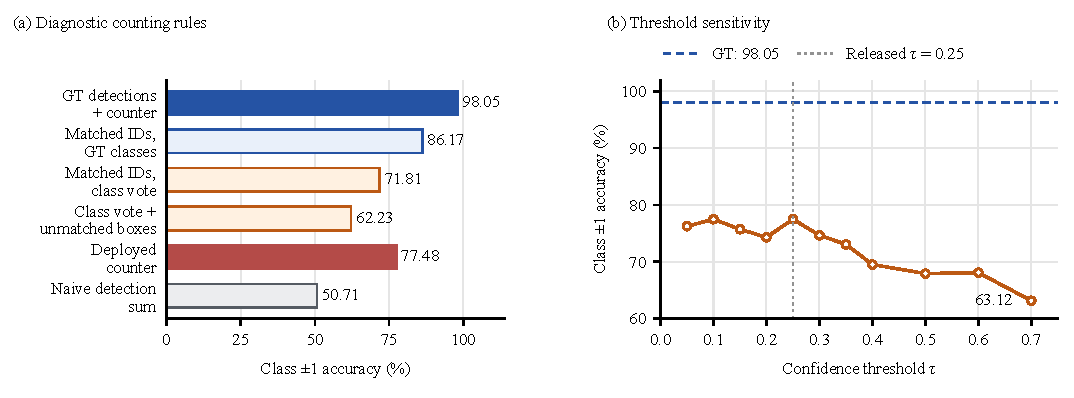
\includegraphics[width=\textwidth]{../figures/paper/fig04_attribution_sweep.pdf}
  \caption{Detection and aggregation diagnostics: (a) six counting rules;
  (b) confidence-threshold sensitivity of Ridge$+F_{\text{all}}$.
  Diagnostic rules are separate estimators, not additive error components.}
  \label{fig:attrib}
\end{figure*}

Figure~\ref{fig:attrib}(a) compares three diagnostic rules. Counting each
matched physical bunch once with its GT class gives 86.17\% Class $\pm$1
Acc. Replacing its GT class by a confidence-weighted vote across matched
detections gives 71.81\%; adding every unmatched detection as a separate
bunch gives 62.23\%. Identity is known only for matched detections, so the
last rule does not deduplicate false positives across views.

The reductions of 13.83 points from exact GT counts to the first rule,
14.36 between the first two rules, and 9.58 between the last two depend on
this ordering, voting rule, and treatment of unmatched detections. They
cannot be added to the GT counter's 1.95-point error to explain the deployed
counter. Indeed, the deployed 77.48\% exceeds two diagnostic rules: learned
aggregation can compensate for systematic detector errors. Likewise,
$86.17-77.48=8.69$ points is a difference between estimators, not an upper
bound on association or counter improvements; the first rule uses GT classes
and removes unmatched detections. The diagnostics expose detection failures,
while the matched-input comparison measures their combined effect on a
specified counting pipeline. Isolating association error itself would require
an implemented association module and controlled interventions on that module.

% ---------------------------------------------------------------------------
\subsection{Sensitivity and Resampling}
\label{sec:robust}

A claim about detector quality drawn from one checkpoint and one split needs
additional checks. Table~\ref{tab:robust} compares a second detector family,
YOLO26 checkpoint capacities, and confidence thresholds.

On the official 141-tree test set, Ridge$+F_0$ reaches 73.76\% Class $\pm$1
and 26.24\% Tree $\pm$1 with YOLO11m, versus 76.06\% and 28.37\% with
YOLO26m. The Class $\pm$1 difference is $-2.30$\,pp (95\% CI
$-4.96$ to $+0.35$, exact $p=0.118$); this does not establish equivalence.
GT reaches 97.70\%, retaining a 23.94-point gap to YOLO11m
(95\% CI 20.57--27.30, $p<0.001$). YOLO11m has 976 unmatched and 399
misclassified appearances out of 2,612 annotations, plus 463 unmatched
detections out of 2,099. Thus the GT advantage extends to this additional
family, without establishing a general architecture ranking.

The operating-point sweep re-runs inference at confidence 0.05 and filters
upward; Ridge$+F_{\text{all}}$ is refitted on the 716 training trees at every
threshold. Raising the threshold from 0.25 to 0.70 reduces Class $\pm$1 Acc
from 77.48\% to 63.12\%. At 0.05, 8,807 test detections yield 76.24\%.
The filtered pass contains 2,353 detections at 0.25 versus 2,354 in the
original cache, with the same reported counting accuracies; the two caches
are not identical. Threshold 0.10 ties 0.25 on Class $\pm$1 and reaches
38.30\% Tree $\pm$1 versus 32.62\%. This is an exploratory test-set sweep,
not independent threshold selection: among these eleven operating points,
none exceeds 77.48\% Class $\pm$1, but the whole-tree endpoint can improve.

On the 64 trees outside gradient training under both split protocols,
Ridge$+F_0$ is fitted on the 590 shared training trees. Class $\pm$1 ranges
from 70.70\% to 73.83\% across four YOLO26 checkpoints, versus 97.27\% for GT:
a 3.13-point checkpoint spread and a 23.44-point GT gap to \texttt{y26mv2}.
This within-family comparison confounds capacity with historical training
splits and includes detector validation trees; it is not an independent
architecture ranking.

Matched $5\times5$-fold CV with Ridge$+F_0$ on the same 237-tree pool gives
$97.72\pm1.02$\% (GT) versus $72.70\pm2.35$\% (fixed), a mean gap of
25.03\,pp. Restricting both conditions to the 141 original test trees gives
$97.16\pm1.23$\% versus $74.08\pm2.96$\%, a 23.08-point gap. These checks
support the ordering with a frozen detector, but their smaller counter
training sets prevent interpreting the original gap as conservative.
For Ridge$+F_{\text{all}}$, counter transfer from DAMIMAS (641 training trees)
to LONSUM (24 evaluation trees) gives 71.88\%, versus 72.92\% when fitted on
LONSUM's 75 training trees. The reverse transfer to 213 DAMIMAS evaluation
trees gives 68.78\%. These comparisons confound estate and counter training
size; the detector saw training trees from both estates.

Vertical-feature sensitivity is tested with the synthetic transformation
$\overline{cy}\mapsto\operatorname{clip}(a\overline{cy}+b,0,1)$ on test
features, with $a\in[0.90,1.10]$ and $b\in[-0.10,0.10]$. Missing-class
sentinels stay at 0.5, and the counter is trained on unperturbed data.
For Ridge$+F_{\text{all}}$, the worst loss is 1.42\,pp; additive Gaussian
noise with $\sigma=0.05$ and seed 42 costs 0.53\,pp. This checks sensitivity
to feature shifts, not physical camera pitch. Actual rotation changes
perspective, box area, visibility, and detector outputs; no calibration or
reacquired pitched images are available to validate those effects.

\begin{table}[!tb]
  \centering
  \footnotesize
  \renewcommand{\arraystretch}{1.13}
  \setlength{\tabcolsep}{3pt}
  \caption{Detector family, checkpoint and threshold sensitivity.}
  \label{tab:robust}
  \begin{tabular*}{\columnwidth}{@{\extracolsep{\fill}}lcccc@{}}
    \toprule
    Setting & Detections & Recall & Class $\pm$1 & Tree $\pm$1 \\
    \midrule
    \multicolumn{5}{@{}l}{\emph{Family, Ridge$+F_0$, 141 test trees}} \\
    YOLO11m            & 2099 & 0.445 & 73.76 & 26.24 \\
    YOLO26m            & 2354 & 0.442 & 76.06 & 28.37 \\
    GT detections      & 2612 & 1.000 & 97.70 & 90.78 \\
    \addlinespace[2pt]
    \multicolumn{5}{@{}l}{\emph{Checkpoint, Ridge$+F_0$, 64 evaluation trees}} \\
    YOLO26n            & 1013 & 0.442 & 72.66 & 34.38 \\
    YOLO26s            &  825 & 0.383 & 72.27 & 26.56 \\
    YOLO26m            &  950 & 0.427 & 70.70 & 28.12 \\
    \texttt{y26mv2}    & 1067 & 0.442 & \textbf{73.83} & 31.25 \\
    GT detections      & 1203 & 1.000 & 97.27 & 89.06 \\
    \addlinespace[2pt]
    \multicolumn{5}{@{}l}{\emph{Operating point, Ridge$+F_{\text{all}}$, 141 test trees}} \\
    $\tau = 0.05$      & 8807 & 0.591 & 76.24 & 34.75 \\
    $\tau = 0.10$      & 5522 & 0.556 & \textbf{77.48} & \textbf{38.30} \\
    $\tau = 0.25$      & 2353 & 0.441 & \textbf{77.48} & 32.62 \\
    $\tau = 0.35$      & 1488 & 0.355 & 73.05 & 23.40 \\
    $\tau = 0.50$      &  799 & 0.245 & 67.91 & 21.28 \\
    $\tau = 0.70$      &  125 & 0.086 & 63.12 & 14.89 \\
    \bottomrule
  \end{tabular*}
\par\vspace{3pt}
  \begin{minipage}{\columnwidth}
    \footnotesize\raggedright
    \textit{Note:} Recall is macro class-correct appearance recall at IoU $\geq0.5$; threshold recall is recomputed after filtering. GT counts are annotated appearances; their recall is 1 by construction.
  \end{minipage}
\end{table}

% ---------------------------------------------------------------------------
\subsection{Why Random Forest Trails}
\label{sec:rf}

RF's Class $\pm$1 deficit relative to ElasticNet and SVM is significant under
GT detections after Holm correction. A plausible explanation is its
prediction range: a forest averages the
training targets reaching each leaf, so its output cannot leave the training
range and is pulled towards the centre of the target distribution wherever a
leaf is thinly populated. Under GT detections the slope of an ordinary
least-squares fit of prediction on truth is 0.754--0.888 across the four
classes for the forest, against 0.865--0.951 for the linear counters, and the
standard deviation of its predictions is a smaller fraction of the true one for
every class. The effect is sharpest where counts are small and the mapping is
close to affine: for B1 the forest never predicts more than three bunches
although the test set holds trees with six, and its MAE is three times that of
Ridge (0.149 against 0.050); the B1 training maximum is only five. In the
highest-load bin it trails ElasticNet by 3.07 points (94.74\% versus
97.81\%). These diagnostics are consistent with shrinkage and sparse
high-count examples, but do not isolate a cause or exclude improvement from
RF tuning. Under the fixed detector, the ElasticNet--RF Class $\pm$1 gap
is unresolved ($p=0.0628$, $p_H=0.628$).

% ---------------------------------------------------------------------------
\subsection{Limitations}
\label{sec:limits}

Several limitations bound these findings. The benchmark uses one dataset of 953
trees from two estates in South Kalimantan, and the smaller estate contributes
99 trees, so cross-site evidence is suggestive rather than conclusive and
absolute numbers may shift under other regions, varieties, or acquisition
protocols. The detector evidence covers YOLO26 and one YOLO11m training run;
software/default differences and the descriptive 64-tree checkpoint comparison
prevent an architecture-only ranking. A plantation excluded from detector
training remains untested. Repeated CV refits counters only; it does not estimate
detector training variability. Camera-pitch robustness remains unverified:
the dataset lacks calibrated pitch measurements or repeated captures at known
angles. Synthetic feature shifts cannot reproduce changes in visibility and
detector output, so spatial-feature findings are limited to the observed
acquisition conditions. Test-based highlighting of configurations limits confirmatory claims;
the validation-selection sensitivity check uses the same historical test set.
The counters treat each tree independently and ignore plantation-scale spatial
or temporal regularities that operational forecasts sometimes exploit. Finally,
the B1 through B4 taxonomy admits genuine visual ambiguity at the B2/B3 and
B3/B4 boundaries. Without inter-annotator measurements we cannot quantify
how much measured confusion arises from label ambiguity. Tree resampling also
does not model spatial dependence among neighbouring trees.

% ---------------------------------------------------------------------------
\section{Conclusion}
% ---------------------------------------------------------------------------

This benchmark compares multi-view tree-level FFB counting under GT boxes and
cached YOLO26m outputs. The best reported Class $\pm$1 scores are 98.05\%
and 77.48\%, a 20.57-point gap (95\% CI 17.20--23.94). The same
Ridge$+F_0$ counter in both conditions retains a 21.63-point gap. No fixed-input
counter pair or Ridge feature addition is significant on Class $\pm$1 after
multiplicity correction, although this does not establish equivalence.
Matched resampling supports the GT advantage, and identity-based diagnostics
reveal substantial missed bunches and class confusion without establishing a
causal error budget or a ceiling on counter improvement.

For automated BBC, these findings favour investigating detector recall and
maturity confusion alongside aggregation, rather than expecting small feature
changes to close the observed gap. Reporting both controlled-input and
detector-input results helps distinguish counter behaviour from the input
quality it receives. Cached detections, tree splits, and evaluation code make
these comparisons reproducible. Per-class and total-count errors further
separate maturity allocation from overall inventory error.

The matched-counter GT advantage also holds for YOLO11m (23.94\,pp).
Evidence remains limited to one dataset, two detector families, and two unequal
estates. Future work should improve B3/B4 detection and B2$\rightarrow$B3
classification, test explicit cross-view association~\cite{ref2,ref3,ref4}
against learned aggregation under matched inputs, and broaden detector evaluation.
An independent plantation, repeated captures at measured camera-pitch angles, and
repeated detector training are needed before extending the conclusion to
other acquisition conditions or operational harvest forecasts.

% ---------------------------------------------------------------------------
\balance
\begin{thebibliography}{00}

\bibitem{ref12}
M.~Kerstan and T.~Fairhurst,
``Use of OMP for accurate crop forecasts,''
Agrisoft Systems and Tropical Crop Consultants Limited. [Online]. Available:
\url{https://www.agrisoft-systems.com/wp-content/uploads/Papers/CropForecastsWithOMPBBC.pdf}.
[Accessed: May 2026].

\bibitem{ref1}
A.~Koirala, K.~B.~Walsh, Z.~Wang, and C.~McCarthy,
``Deep learning: method overview and review of use for fruit detection and
yield estimation,''
\textit{Computers and Electronics in Agriculture}, vol.~162, pp.~219--234,
Jul.~2019, doi: 10.1016/j.compag.2019.04.017.

\bibitem{ref5}
M.~Stein, S.~Bargoti, and J.~Underwood,
``Image based mango fruit detection, localisation and yield estimation using
multiple view geometry,''
\textit{Sensors}, vol.~16, no.~11, Art. no.~1915, Nov.~2016,
doi: 10.3390/s16111915.

\bibitem{ref6}
P.~Roy, A.~Kislay, P.~A.~Plonski, J.~Luby, and V.~Isler,
``Vision-based preharvest yield mapping for apple orchards,''
\textit{Computers and Electronics in Agriculture}, vol.~164, Art. no.~104897,
Sep.~2019, doi: 10.1016/j.compag.2019.104897.

\bibitem{ref7}
N.~H\"{a}ni, P.~Roy, and V.~Isler,
``A comparative study of fruit detection and counting methods for yield
mapping in apple orchards,''
\textit{Journal of Field Robotics}, vol.~37, no.~2, pp.~263--282, Mar.~2020,
doi: 10.1002/rob.21902.

\bibitem{ref3}
M.~Gaillard, B.~Benes, M.~C.~Tross, and J.~C.~Schnable,
``Multi-view triangulation without correspondences,''
\textit{Computers and Electronics in Agriculture}, vol.~206, Art. no.~107688,
Mar.~2023, doi: 10.1016/j.compag.2023.107688.

\bibitem{ref4}
H.~Freeman, E.~Schneider, C.~H.~Kim, M.~Lee, and G.~Kantor,
``3D reconstruction-based seed counting of sorghum panicles for agricultural
inspection,''
in \textit{Proc. IEEE International Conference on Robotics and Automation
(ICRA)}, 2023, pp.~9594--9600, doi: 10.1109/ICRA48891.2023.10161400.

\bibitem{ref8}
L.~Meyer, A.-T.~Ardelean, T.~Weyrich, and M.~Stamminger,
``FruitNeRF++: A generalized multi-fruit counting method utilizing contrastive
learning and neural radiance fields,''
in \textit{Proc. IEEE/RSJ International Conference on Intelligent Robots and
Systems (IROS)}, 2025, pp.~1717--1724, doi: 10.1109/IROS60139.2025.11247341.

\bibitem{ref14}
C.-Y.~Wang, A.~Bochkovskiy, and H.-Y.~M.~Liao,
``YOLOv7: Trainable bag-of-freebies sets new state-of-the-art for real-time
object detectors,''
in \textit{Proc. IEEE/CVF Conference on Computer Vision and Pattern
Recognition (CVPR)}, 2023, pp.~7464--7475,
doi: 10.1109/CVPR52729.2023.00721.

\bibitem{ref15}
G.~Jocher and J.~Qiu,
``Ultralytics YOLO26,'' Ultralytics, 2026. [Software].
Available: \url{https://github.com/ultralytics/ultralytics}.

\bibitem{refNaftali2024}
M.~G.~Naftali, G.~Hugo, and Suharjito,
``Palm oil counter: State-of-the-art deep learning models for detection and
counting in plantations,''
\textit{IEEE Access}, vol.~12, pp.~90395--90417, 2024,
doi: 10.1109/ACCESS.2024.3419835.

\bibitem{ref9}
N.~A.~Prasetyo, Pranowo, and A.~J.~Santoso,
``Automatic detection and calculation of palm oil fresh fruit bunches using
Faster R-CNN,''
\textit{International Journal of Applied Science and Engineering}, vol.~17,
no.~2, pp.~121--134, 2020, doi: 10.6703/IJASE.202005\_17(2).121. [Online]. Available:
\url{https://gigvvy.com/journals/ijase/articles/ijase-202005-17-2-121}

\bibitem{ref10}
J.~W.~Lai, H.~R.~Ramli, L.~I.~Ismail, and W.~Z.~W.~Hasan,
``Real-time detection of ripe oil palm fresh fruit bunch based on YOLOv4,''
\textit{IEEE Access}, vol.~10, pp.~95763--95770, 2022,
doi: 10.1109/ACCESS.2022.3204762.

\bibitem{ref11}
M.~Y.~M.~A.~Mansour, K.~D.~Dambul, and K.~Y.~Choo,
``Object detection algorithms for ripeness classification of oil palm fresh
fruit bunch,''
\textit{International Journal of Technology}, vol.~13, no.~6,
pp.~1326--1335, 2022, doi: 10.14716/ijtech.v13i6.5932.

\bibitem{ref13}
M.~H.~Junos, A.~S.~M.~Khairuddin, S.~Thannirmalai, and M.~Dahari,
``Automatic detection of oil palm fruits from UAV images using an improved
YOLO model,''
\textit{The Visual Computer}, vol.~38, no.~7, pp.~2341--2355, 2022,
doi: 10.1007/s00371-021-02116-3.

\bibitem{refSuharjito2025}
Suharjito, M.~G.~Naftali, G.~Hugo, M.~R.~A.~Priyadi, M.~Asrol, and
D.~N.~Utama,
``Oil palm fruits dataset in plantations for harvest estimation using digital
census and smartphone,''
\textit{Scientific Data}, vol.~12, p.~972, Jun.~2025,
doi: 10.1038/s41597-025-05227-x.

\bibitem{refIndriani2026}
F.~Indriani et al.,
``SawitMVC: A Multi-View Oil Palm Fruit Bunch Dataset for Detection and
Counting,'' Zenodo, May~22, 2026,
doi: 10.5281/zenodo.20336323.

\bibitem{ref16}
T.-Y.~Lin et al.,
``Microsoft COCO: Common objects in context,''
in \textit{Proc. European Conference on Computer Vision (ECCV)}, 2014,
pp.~740--755, doi: 10.1007/978-3-319-10602-1\_48.

\bibitem{ref19}
A.~E.~Hoerl and R.~W.~Kennard,
``Ridge regression: Biased estimation for nonorthogonal problems,''
\textit{Technometrics}, vol.~12, no.~1, pp.~55--67, 1970,
doi: 10.1080/00401706.1970.10488634.

\bibitem{ref17}
H.~Zou and T.~Hastie,
``Regularization and variable selection via the elastic net,''
\textit{Journal of the Royal Statistical Society B}, vol.~67, no.~2,
pp.~301--320, 2005, doi: 10.1111/j.1467-9868.2005.00503.x.

\bibitem{ref20}
C.~Cortes and V.~Vapnik,
``Support-vector networks,''
\textit{Machine Learning}, vol.~20, no.~3, pp.~273--297, 1995,
doi: 10.1007/BF00994018.

\bibitem{ref18}
L.~Breiman,
``Random forests,''
\textit{Machine Learning}, vol.~45, no.~1, pp.~5--32, 2001,
doi: 10.1023/A:1010933404324.

\bibitem{ref2}
X.~Liu, S.~W.~Chen, C.~Liu, S.~S.~Shivakumar, J.~Das, C.~J.~Taylor,
J.~Underwood, and V.~Kumar,
``Monocular camera based fruit counting and mapping with semantic data
association,''
\textit{IEEE Robotics and Automation Letters}, vol.~4, no.~3, pp.~2296--2303,
Jul.~2019, doi: 10.1109/LRA.2019.2901987.

\end{thebibliography}

\end{document}
